\chapter{Calibration of the electromagnetic calorimeter}
\label{sec:org3ad4877}
\label{sec:Calibration_calibration}
\section{Overview}
\label{sec:orgd33fdfe}

Electromagnetic particles (electrons and photons) are heavily used in precision measurements due to the high precision reachable by (the tracker and) the electromagnetic calorimeter.
In particular, the measurement of the properties of the Higgs boson will be a major goal for run 2.
As for the discovery, the (at least partially) electromagnetic channels ( $H\rightarrow\gamma \gamma$ and H\(\rightarrow\) 4l ) will play a major role.
Measuring the mass of the W boson down to 19 MeV of uncertainty has also been performed at 7 TeV \cite{CERN-EP-2016-305} and has interesting prospects at 13 TeV.
To reach such a precision in property measurements, a precise calibration of the energy of electrons and photons is required.

The calibration procedure starts with the raw energy of the reconstructed objects.
It relies on a multivariate analysis (MVA), per trained on a full simulation of the detector in GEANT4 \cite{GEANT4}.
Several in-situ analyses are also performed to evaluate and correct effects inaccurately simulated.
Fig. \ref{fig:orgfcfa421} shows the flowchart of the calibration, with the respective paths of data and MC.
The data must first pass an analysis which determines the amount of passive material in front of the ECAL using the longitudinal energy distribution of electrons and photons.
This study corrects for the possible mismodellings of the detector geometry, where the inner detector part of this geometry has been optimised using hadronic interactions and photon conversion vertices \cite{CERN-EP-2017-081}.
Once the geometry has been validated, the MC is passed through it and the detector response is used to train a MVA separately for unconverted photons, converted photons and electrons.
The energy calibration of data is then performed using the trained MVA.
Finally, when comparing data and MC distributions of the Z\(\rightarrow\) ee invariant mass, we observe a discrepancy.
A $Z\rightarrow ee$ in-situ analysis computes correction factors to be applied both on data and MC to match the distributions.
Energy scale factors shift the energy of data events in order to align data and MC Z mass distribution.
Resolution constant terms are used to smear the MC in order to match the widths of the distributions.
Finally cross-checks are performed on other physics processes to support the quality of the calibration procedure.

\begin{figure}[htbp]
\centering
\includegraphics[width=\linewidth]{Calibration_1f.pdf}
\caption{\label{fig:orgfcfa421}
Schematic overview of the calibration procedure of electromagnetic particles in ATLAS.\cite{CERN-PH-EP-2014-153}}
\end{figure}


\section{Multivariate calibration}
\label{sec:org8232c38}

The multivariate calibration \cite{CERN-PH-EP-2014-153,ATL-COM-PHYS-2013-1426,ATL-COM-PHYS-2017-761} is the central component of the ATLAS procedure to calibrate the energy of electrons and photons.
It replaces the original calibration \cite{ATL-LARG-PUB-2007-012} which relied on the functional parametrization of the energy as a function of a set of input variables.
The multivariate technique allows for a more simple implementation.
It relies on machine learning to find the best combination of input variables to minimize the RMS of a target variable.
In practice, a boosted decision tree (BDT) from the TMVA package \cite{physics/0703039,CERN-OPEN-2007-007} has been chosen.
The ratio E\(^{\text{corr}}\)/E\(^{\text{true}}\) has been chosen as target variable as showing the best compromise between BDT optimal setup and physics meaning.
Because of the detector inhomogeneity along $\eta$ and the difference of detector response as a function of energy, a binning in $|\eta_\text{cluster}|$ and $E_T$ has been performed leading to 102 configurations to optimize independently.
The optimization was further splitted between electrons, converted and unconverted photons.
Due to their similar behaviour, electrons and photons correction factors are trained on a common set of variables, sensitive to specific effects :

\begin{itemize}
\item E\(_{\text{acc}}\) : the total energy measured in the accordion defined as the uncalibrated sum of energies in each layer (strips, middle and back ).
\item E\(_{\text{0}}\)/E\(_{\text{acc}}\) : the ratio of the energy in the presampler over the energy in the accordion. This variable is used only for $|\eta|<1.8$ (zone where there is the pre-sampler).
\item \(X=\sum X_iE_i / \sum E_i\) : the longitudinal shower development where X represents the amount of material in unit of $X_0$ in each calorimeter layer or in front of the presampler.
  For run 2, X is replaced by the ratio of the uncalibrated energy in the first over the second layer ($E_1/E_2$).
\item \(\eta_{\text{cluster}}\) : the pseudo rapidity in the ATLAS frame, taking into account the misalignment of the detector to precisely correct for geometry effects.
\item Cell index : an integer number defined as the integer part of the division ( \(\eta_{\text{calo}}\)/\(\Delta \eta\)) where \(\eta_{\text{calo}}\) is the cluster pseudo rapidity in the calorimeter frame with \(\Delta \eta\) as the size of one cell in the middle layer. This variable is also sensitive to the geometry non-uniformities.
\item $\eta$ position of the cluster with respect to the cell edge.
This variable is defined as the pseudorapidity in the calorimeter frame modulus the width of one cell of the middle layer (\(\Delta \eta\)).
It is sensitive to the lateral leakage of the cluster.
\item $\phi$ with respect to the lead absorber. This variable is sensitive to the modulation of the thickness of the absorber as a function of $\phi$.
\end{itemize}


Converted photons, defined by having a conversion radius $0<R<800$ mm,  do not have uniform sensitivity to material along their path.
Additional variables are included into the BDT to include this inhomogeneity in the optimization :


\begin{itemize}
\item R : Radius of conversion. This variable is used only if the $p_T$ sum of the conversion tracks is above 3 GeV. The radius is set to 799 mm otherwise.
\item E\(^{\text{acc}}_{\text{T}}\)/$p_T$ : Ratio of the transverse energy in the accordion with respect to the conversion $p_T$. This variable is set to 2 in the case of single track converted photons or if at least one track has no hit in the silicon detector.
\item p\(_{\text{T}}^{\text{High}}\)/p\(_{\text{T}}^{\text{conv}}\) : Fraction of $p_T$ carried by the highest $p_T$ track of a conversion. It is set to 1 in case of non Si-Si tracks.
\end{itemize}


One can observe that no variable related to the lateral shower shape is included in the BDT.
While being promising in term of added information, this shape is inaccurately simulated in MC so is not included.
A challenge of run 2 is to better understand the shower shape discrepancies and to include them in the MVA later on.

\begin{figure}[htbp]
\centering
\includegraphics[width=0.6\linewidth]{ATL-COM-PHYS-2013-1426_3f.pdf}
\caption{\label{fig:org7143a4c}
Distribution of the target variable of the calibration BDT E\(^{\text{corr}}\)/E\(^{\text{true}}\) for electrons in a representative bin in run 1. The distribution of the original calibration and MVA before and after energy shifts are compared. \cite{ATL-COM-PHYS-2013-1426}}
\end{figure}


As mentionned earlier, the BDT targets the minimization of the RMS of E\(^{\text{corr}}\)/E\(^{\text{true}}\) but not its central value.
This condition imposes the maximum of the distribution to be close to 1 but not exactly, which was the target of the original calibration as can be shown in fig. \ref{fig:org7143a4c}.
A second correction, in the form of an energy scale is applied post MVA to set the most probable value of the distribution to 1.
This additional correction is observed to have significant differences from bin to bin.
The binning in $E_T$ has then been changed for this correction in order to improve the continuity of the correction shifts and to perform a linear fit as a function of $E_T$.
The average between the two methods, with inflated uncertainties to take into account their difference, is used later for the correction.

The final peak position and resolution for run 1 as a function of $\eta$, E and particle type are shown in fig. \ref{fig:orgd9949ea}.
The most probable value corresponds to the central value of a gaussian fitted in the range [-1,2] standard deviations around the maximum of the  E\(^{\text{corr}}\)/E\(^{\text{true}}\) distribution.
The resolution is computed as the interquartile of the distribution, renormalized to its definition for a gaussian.

\begin{figure}[htbp]
\centering
\includegraphics[width=0.9\linewidth]{CERN-PH-EP-2014-153_2f.pdf}
\caption{\label{fig:orgd9949ea}
MC energy MPV and resolution after run1 MVA calibration as a function of $\eta$ for different energy bins and particle types.\cite{CERN-PH-EP-2014-153}}
\end{figure}

Once trained, the multivariate corrections are applied on MC and data reconstructed events.

\section{Layer intercalibration}
\label{sec:org0cd5325}


The MVA optimization relies on the assumption that the electronic and geometric description of the detector are perfect.
Known discrepancies between data and simulation are then to be corrected before applying MVA correction to the data.
Residual mis-calibration of the cells lead to overall discrepancies in the cluster energy for each layer.
First the relative response between layers 1 and 2 of the ECAL is corrected.
It allows then to evaluate the corrections on the presampler energy response.

\subsection{ECAL layers inter-calibration}
\label{sec:org9663735}

Muons are ideal probes for layer inter-calibration \cite{ATL-COM-PHYS-2013-1423,ATL-COM-PHYS-2017-760} of the accordion as their energy deposit is very localized in one or two cells.
The critical energy in the presampler and the ECAL is about 100 GeV, which make muons from Z decay minimum ionizing particle.
The total energy deposit in a layer of active material is then a measure of the amount of liquid argon crossed by the muon.
Similarly, the muons have a low sensitivity to the material they cross, so muon inter-calibration is independent of the quantity of matter in front of the calorimeter.

Due to the low energy deposit from muons in calorimeter cells, there is a significant contribution of electronic and pile-up noise in the energy response.
Its distribution is described as a Landau function for the physical process convoluted with a gaussian distributed noise.
Two methods are compared to extract the MPV (Most Probable Value) of the distribution : a direct fit of the distribution by the convolution or a truncated mean.
The truncated mean consists in finding the smallest interval containing X\% of the events and computing its mean.
While this method does not extract directly the MPV, the mean is strongly correlated to it so comparison between data and MC is possible.

The cross talk between cells in the first layer of the ECAL is not well described in the MC and has non-negligible effects.
Averaging the cross talk using several cells allows for a better comparison with simulation hence the energy deposit of muons in the layer 1 (L1) is defined as the sum of the highest energy cell and its two neighbours in $\eta$ since the size of the cells in L1 in $\phi$ is much larger.
The L2 has a smaller cross-talk but accordion geometry of the L2 leads muons to cross several cells in $\phi$ on its trajectory.
For a better determination of the energy deposit, the sum of the central cell and its highest energy neighbour are summed since run 2.

The ratio E\(_{\text{1/2}}\) of the MPV of L1 energy deposit over the L2  in data is compared with the simulation in |$\eta$| bins, as no significant discrepancy was observed between negative and positive $\eta$.
The result, presented in fig. \ref{fig:orgbc717bb}, shows a behaviour of the double ratio with several structures.
In particular, one can observe the detector substructure with up to 5\% shifts at |$\eta$|=0.8 and in the crack.

Two ways are possible to correct for this discrepancy : one can rescale the energy of the data events either in the L1 or in the L2 in the data to retrieve agreement with MC.
A study showed that the L2 energy contributed more in the observed pattern so it was decided to rescale E\(_{\text{2}}\).
After all corrections have been applied, the particle energy is independent of this choice.

\begin{figure}[htbp]
\centering
\includegraphics[width=0.9\linewidth]{CERN-PH-EP-2014-153_12f.pdf}
\caption{\label{fig:orgbc717bb}
Ratio of E\(_{\text{1/2}}^{\text{data}}\)/E\(_{\text{1/2}}^{\text{MC}}\) as a function of |$\eta$| for run 1.\cite{CERN-PH-EP-2014-153}}
\end{figure}

\subsection{Presampler inter-calibration}
\label{sec:org3279565}

The presampler (PS) scale  factor is evaluated comparing the data and MC distributions of the energy (E\(_{\text{0}}\)) deposited by electrons from W and Z decays.
Because electrons are considered in this analysis, a discrepancy of the energy distributions between data and MC can arise due to cell miscalibration, which has to be corrected, but also from material mismodelling upstream of the PS.
The expected correlation between E\(_{\text{0}}\) and E\(_{\text{1/2}}\) for electrons is used to remove the material contribution.
Indeed, with an increase of material, the electron EM shower will start earlier and have a higher PS energy deposit and will also deposit more energy in the L1, hence increasing E\(_{\text{1/2}}\).
Furthermore, an increase of material between the PS and the ECAL will also increase E\(_{\text{1/2}}\) without any impact on E\(_{\text{0}}\).

To study the correlation between E\(_{\text{0}}\) and E\(_{\text{1/2}}\) including the material effects, MC samples have been generated with modified geometries with increased material in different detector subsystems.
For each of these samples, the MPV of the presampler energy E\(_{\text{0}}^{\text{var}}\) and E\(_{\text{1/2}}^{\text{var}}\) (var meaning various simulations) are compared to their respective values for the nominal geometry ( E\(_{\text{0}}^{\text{MC}}\) and E\(_{\text{1/2}}^{\text{MC}}\)).
The results are shown in fig. \ref{fig:orgb8e95bb} for a typical $\eta$ bin.
One observe that all the variations of material upstream of the PS are aligned, hence describing a linear correlation between the double ratios.
A similar correlation with an offset along E\(_{\text{1/2}}\) is observed when adding material between the PS and the ECAL.
A linear parametrization of the correlation is performed in each $\eta$ bin and a global parametrization as a function of $\eta$ is defined,

\begin{equation}
\label{eq:orgf855cf3}
\frac{E_0^{var}}{E_0^{MC}} = 1 + A(\eta) \left( \frac{E_{1/2}^{var}}{E^{MC}_{1/2}b_{1/2}}(\eta) -1 \right)
\end{equation}

with : A($\eta$) describing the impact of the ID  material budget upstream of the PS (i.e. the slope of fig. \ref{fig:orgb8e95bb}), b\(_{\text{1/2}}\) a correction for discrepancy in the electron E\(_{\text{1/2}}\) distribution between data and MC due only to effects downstream of the PS.
Cross-talk mismodelling or material discrepancy between the PS and the accordion affect similarly the electrons and the photons hence a sample of unconverted photons is used to measure b\(_{\text{1/2}}\).
A veto on the PS activity is performed to reduce the probability of a conversion between the ID and  the PS, which leads to minimal sensitivity to material in front of the PS.

Using b\(_{\text{1/2}}\) and E\(_{\text{1/2}}^{\text{data}}\) from data, one can compute the expected E\(_{\text{0}}^{\text{corr}}\) energy deposit in the PS in the data.
A is obtained by fitting the correlation in fig. \ref{fig:orgb8e95bb} with eq. \ref{eq:orgf855cf3}.
Finally, the correction factor on the PS energy is defined as \(\alpha_{\text{PS}}\)($\eta$)=E\(_{\text{0}}^{\text{data}}\)/E\(_{\text{0}}^{\text{corr}}\).
The ratio of PS energy in data over MC is shown in fig. \ref{fig:org73e96b5} before and after the correction.
The remaining miscalibration of the PS have been reduced down to 5\% in the barrel applying the procedure in eq. \ref{eq:orgf855cf3}.
The larger difference before is mostly related to differences in material before the calorimeter between data and simulation.


\begin{figure}[htbp]
\centering
\includegraphics[width=0.9\linewidth]{CERN-PH-EP-2014-153_13fa.pdf}
\caption{\label{fig:orgb8e95bb}
Correlation between E\(_{\text{0}}\) and E\(_{\text{1/2}}\) for run 1, 0.6<|$\eta$|<0.8, and different material variations upstream of the ECAL. Variations refer to addition of material up to 15\% $X_0$ in the ID and/or between the PS and the ECAL. Correlation parameters from eq. \ref{eq:orgf855cf3} fitted values are displayed. \cite{CERN-PH-EP-2014-153}}
\end{figure}


\begin{figure}[htbp]
\centering
\includegraphics[width=0.9\linewidth]{CERN-PH-EP-2014-153_15f.pdf}
\caption{\label{fig:org73e96b5}
Ratio of presampler energy MPV between data and MC before and after correction of b\(_{\text{1/2}}\) and material upstream of the PS. \cite{CERN-PH-EP-2014-153}}
\end{figure}


\section{In situ Z\(\rightarrow\) ee calibration}
\label{sec:org48e1333}
\label{sec:Calibration_inSituZee}

\subsection{Overview}
\label{sec:org5e89c11}

The calibration procedure so far is not enough to recover a perfect energy response.
Other unknown or complicated phenomena, such as OFC residual discrepancies, remain.
A bias in the reconstructed energy of data is observed with respect to the simulation.
The mass distribution of the Z in the electronic decay channel is shown in fig. \ref{fig:orgb935e5f} and a large discrepancy is observed between the data and the simulation.
This discrepancy is however partly due to the choice of applying the $E_1/E_2$ on the L2.

To ensure good performances in spite of the wide variety of possible effects, a data driven correction is derived  using the well known Z mass \cite{PDG2016} as a reference \cite{ATL-LARG-2004-008,ATL-COM-PHYS-2013-1653}.
These corrections shift the data distribution with an energy scale factor \(\alpha\) and enlarge the MC distribution with an additional resolution constant term c to reach the best agreement between the distributions.
In order to better match detector in-homogeneities, hence improving the resolution, the corrections are measured in $\eta$ bins.


\begin{figure}[htbp]
\centering
\includegraphics[width=0.9\linewidth]{CalibSupNote_Distri_m12_uncorrected.pdf}
\caption{\label{fig:orgb935e5f}
Data and MC Z mass distribution before final in-situ calibration.}
\end{figure}


The energy scale factor is a multiplicative correction on the energy of an electron (or photon).
It is designed to correct the global calorimeter energy scale.
The definition of \(\alpha\) follows eq. \ref{eq:org4f3fdd9}, where \(E^{rec}\) is the measured reconstructed electron energy and \(E^{corr}\) is the corrected energy, emulating the true energy.
It is measured by modifying the MC to match the data but is applied on data to match the MC (in order to improve the resolution on data).
A positive value means that the electron energy has been overestimated in the calibration procedure.
Eq.  \ref{eq:org66bdacb} presents how correcting electrons energy affects the Z mass.
In the case of identical corrections for both electrons, it is equivalent to directly correct the mass by \(\alpha\).

\begin{equation}
\label{eq:org4f3fdd9}
E^{corr}=\frac{E^{rec}}{1+\alpha}
\end{equation}

\begin{equation}
\label{eq:org66bdacb}
M_Z^{corr} =  \frac{M_Z^{rec}}{\sqrt{(1+\alpha_1)(1+\alpha_2)}} \simeq \frac{M_Z^{rec}}{1+\frac{\alpha_1+\alpha_2}{2}} = \frac{M_Z^{rec}}{1+\alpha_{12}}
\end{equation}


It is observed that the width of the data is larger than the one of the MC.
This can be due to in-homogeneous effects affecting linearly the energy, or to the contribution of random energy fluctuations.
This increase is assumed to be described by a Gaussian convolution.
The total detector resolution can then be parametrized as :

\begin{equation}
\label{eq:orgba2e3cd}
  \frac{\sigma}{E} = \frac{a}{\sqrt{E}} \oplus \frac{b}{E} \oplus c' \oplus c = \left(\frac{\sigma}{E}\right)_{MC} \oplus c
\end{equation}

with $a$ ($\sim300$ MeV) the stochastic term related to shower fluctuations in the LAr and modelled by simulation, $b$ ($10\%$) the electronic and pile-up noise term measured every morning on dedicated runs, $c'$ the intrinsic constant term of the Monte-Carlo and $c$ the additional one.
The detector design and calibration procedure aimed at maintaining the additional constant term to below 1\%.
The additional constant term correction, later referred simply as constant term, is applied on all electrons and photons.
It is implemented by multiplying the energy of the particle by (1+rc), with r a random number generated on a normal distribution.
This procedure is slightly different than an analytic Gaussian convolution of the mass distribution.
However, one has the opportunity to apply different corrections  on each electron.

Contrary to \(\alpha\) there is no direct relation between the applied correction c and the corrected resolution.
A relation only appears on average when considering the width of the full corrected and uncorrected distributions.
The effective constant term of the corrected Z mass distribution will be related to the correction factors of both electrons in the $\eta$ bins 1 and 2 according  to eq. \ref{eq:orgb4e7ae0} since~:

\begin{equation}
\begin{array}{lll}
\left( \frac{\sigma(m)}{m} \right)^2 &\simeq& \frac{1}{4}\left( (\frac{\sigma(E_1)}{E1})^2 + (\frac{\sigma(E_2)}{E_2})^2 \right)\\
& = &\frac{1}{4}\left( (\frac{\sigma(E_1)}{E1})_{MC}^2 + c_1^2 + (\frac{\sigma(E_2)}{E_2})_{MC}^2+ c^2_2 \right)\\
& = &\left( \frac{\sigma(m)}{m} \right)_{MC}^2 + \frac{c_1^2+c_2^2}{4}\\
\end{array}
\end{equation}

If one considers instead the effective correction c\(_{\text{12}}\) to apply on both electrons (with independent random numbers), the resolution takes the form :


\begin{equation}
\left( \frac{\sigma(m)}{m}\right)^2 = \left( \frac{\sigma(m)}{m}\right)_{MC}^2 + \frac{c_{12}^2 + c_{12}^2}{4} = \left( \frac{\sigma(m)}{m}\right)_{MC}^2 + \frac{c_{12}^2}{2}
\end{equation}

Finally one has :

\begin{equation}
\label{eq:orgb4e7ae0}
  c_{12}^2=\frac{c_1^2+c_2^2}{2}
\end{equation}
Using this formula allows to relate the effective quadratic difference of the RMS of two distributions to the corrections of individual electrons.

\subsection{Selection and corrections}
\label{sec:org472930d}

Events are selected containing exactly two electrons of opposite charges.
Electrons candidates must pass the triggers HLT\_2e12\_lhloose\_L12EM10VH and HLT\_2e17\_lhvloose\_nod0 for 2015 and 2016 data respectively.
For precise measurement, a reconstruction quality is required on them : they must have at least a medium tag from the offline identification algorithm.
Another selection removes the electrons which fall into bad regions of the detector.
A loose isolation cut is applied to further reduce the QCD background.
The vertex position along z of the event must be below 150 mm.
The data must further be in the good run list which is a list of  time periods in which the detector was fully operational.
A cut flow of this selection is presented in fig. \ref{fig:org0348ce0}.
This thesis presents the central electron calibration requesting $|\eta|<2.47$.
A larger $|\eta|$, the absence of tracker and the increased background changes the paradigm of the analysis.
A dedicated measurement is performed in the forward region, using the results from central electrons.
As forward electrons are not used in precision measurement, no further description of the forward analysis is performed.

\begin{figure}[htbp]
\centering
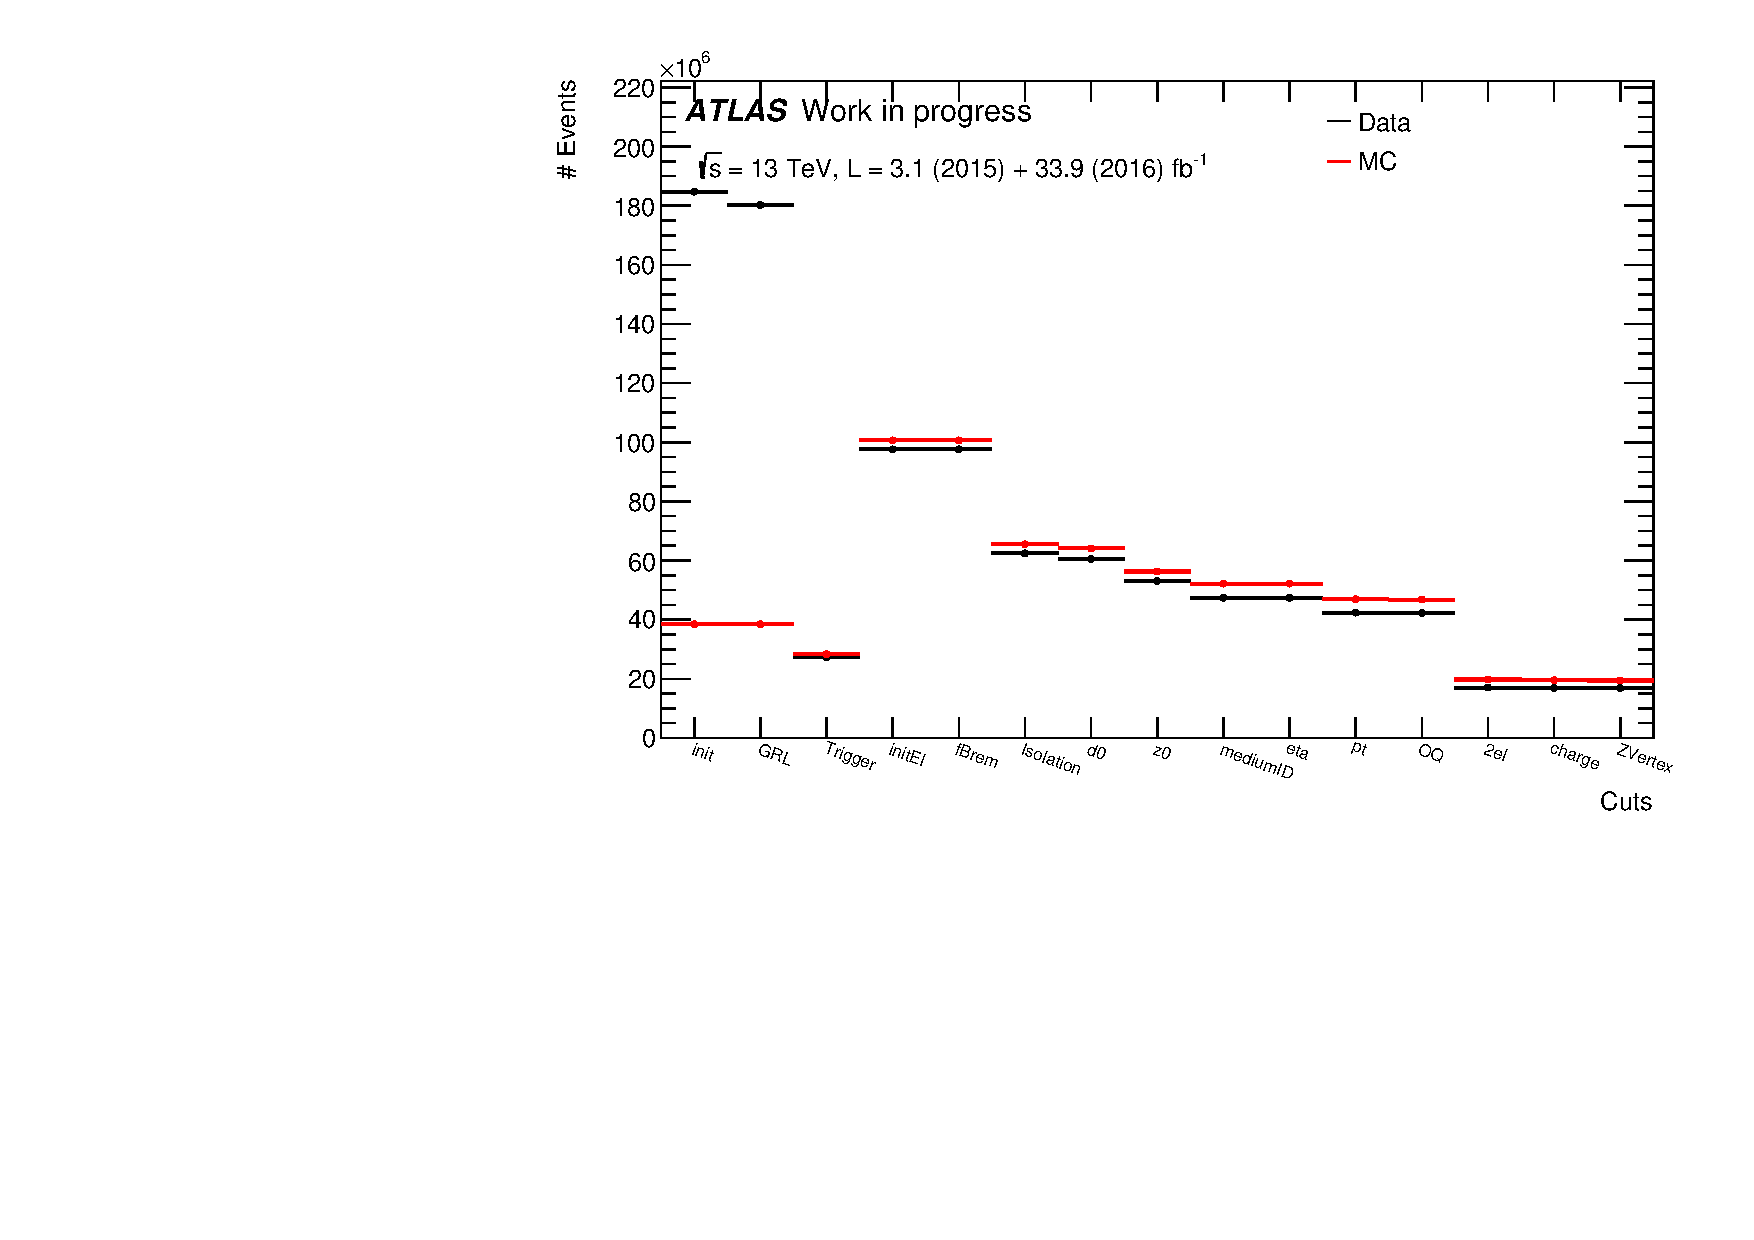
\includegraphics[width=0.9\linewidth]{Figures/cutFlow.pdf}
\caption{\label{fig:org0348ce0}
Comparison of cutflow for data and MC $Z\rightarrow ee$ samples.}
\end{figure}

The results presented in this thesis use the full 2015+2016 data with an integrated luminosity of 36.1 fb\(^{\text{-1}}\) for a total of 17 million events in the Zee sample.
80 millions MC events have been generated using Powheg and Pythia for the shower development.
Their interaction with the detector is simulated using a full GEANT4 \cite{GEANT4} detector geometry and the full reconstruction and calibration algorithms.
After selection 19 millions MC events are used for the scale measurement.

Corrections must be applied to both data and MC in the form of weights on the events.
Selection efficiencies of the different reconstruction steps are not the same in data and MC.
Reweighting factors for trigger, reconstruction, isolation and identification efficiencies are applied only on the MC.
Reconstruction and identification have a pile-up dependence.
MC events are reweighted so that their pile-up distributions match the data distribution.
The simulated Z mass shape modification due to the reweightings is shown in fig. \ref{orgb5c10cf}.

\begin{figure}
\begin{subfigure}[t]{\linewidth}
\begin{center}
\includegraphics[width=0.7\linewidth]{CalibSupNote_compWeight_m12_SF.pdf}
\end{center}
\end{subfigure}
\begin{subfigure}[t]{\linewidth}
\begin{center}
\includegraphics[width=0.7\linewidth]{CalibSupNote_compWeight_m12_PU.pdf}
\end{center}
\end{subfigure}
\caption{\label{orgb5c10cf}
Modification of the simulated Z mass shape due to reweightings. Efficiency scale factors are shown on the top plot while pile-up reweightings on the bottom plot.}
\end{figure}

\subsection{Binning}

  The detector is not homogeneous as a function of $\eta$ as can be seen in fig. \ref{fig:org37061bb} which shows an overview of the material budget in the inner detector.
  As a result, the performances of the detector are themselves function of $\eta$.
  It is then necessary to measure calibration constants which reflect those in-homogeneities.
  In order to have a fine correction, hence a better final resolution, the correction measurement is performed in $\eta$ bins.
  The variable $\eta_{\text{calo}}$ is chosen as the most related to the calorimeter structures.
  With this methodology, it is assumed that all electrons of a bin should have the same correction, which requires small $\eta$ bins.
  The differences with respect to this assumption will effectively increase the measured additional constant term, hence should be corrected at first order.
  For run 1 \cite{CERN-PH-EP-2014-153}, the calorimeter was splitted in 34 regions for the measurement of the energy scales, and 24 bins (symmetrized) for the resolution constant terms.
  For run 2, 68 bins have been defined for \(\alpha\), corresponding roughly to the bins of run 1 splitted in two.
  This increase have been decided at the beginning of run 2 after the observation of patterns in the scales (more in section \ref{sec:org6c03620}).
  For the constant term, the binning of run 1 was kept, but slightly modified in order to take into account the change of variable from $\eta_\text{tracker}$ to $\eta_\text{calo}$.
  The bins edges are shown in table \ref{tab:Calibration_inSitu_binning}.

\begin{figure}[htbp]
\centering
\includegraphics[width=0.9\linewidth]{CERN-LHCC-2010-013_13fc.pdf}
\caption{\label{fig:org37061bb}
Material budget in front of the electromagnetic calorimeter of the ATLAS detector.\cite{CERN-LHCC-2010-013}}
\end{figure}


\begin{table}
\caption{Absolute values of $\eta_{calo}$ bin edges for energy scale factors (black and brown) and resolution constant terms (brown) for run~2.}
\label{tab:Calibration_inSitu_binning}
\resizebox{\linewidth}{!}{%
\begin{tabular}{c}
\textcolor{brown}{0}  0.1  \textcolor{brown}{0.2}  0.3  \textcolor{brown}{0.4}  0.5  \textcolor{brown}{0.6}  0.7  \textcolor{brown}{0.8}  0.9  \textcolor{brown}{1}  1.1  \textcolor{brown}{1.2}  1.285  \textcolor{brown}{1.37}  1.42  1.47  1.51  \textcolor{brown}{1.55}  1.59  1.63  1.6775  1.725  1.7625  \textcolor{brown}{1.8}  1.9  \textcolor{brown}{2}  2.05  2.1  2.2  \textcolor{brown}{2.3}  2.35  2.4  2.435  \textcolor{brown}{2.47} \\
\end{tabular}
}
\end{table}


Considering N\(_{\text{B}}\) $\eta$ bins for electrons, there exist N\(_{\text{B}}^{\text{2}}\) number of electron pair configurations for a Z boson.
This amount decreases to \(N_{conf}=\frac{N_B(N_B+1)}{2}\) when removing the ordering of the electrons.
Z events are then categorized into  N\(_{\text{conf}}\) configurations (i,j) in which the template method is used.
By injecting the same \(\alpha\) and c for both electrons at the template creation, the template method only allows to measure the effective \(\alpha_{\text{ij}}\) or c\(_{\text{ij}}\) necessary to match the data and MC.
Eq. \ref{eq:org66bdacb} and \ref{eq:orgb4e7ae0} allow to relate the effective correction in a configuration to the real correction of each electrons.
By combining the equations from the N\(_{\text{conf}}\) configurations, the measurement of the N\(_{\text{B}}\) corrections terms (\(\alpha\) or c) is possible.
The combination is later referred as the inversion.


% \begin{equation}
% \label{eq:orgc99789a}
% \begin{array}{l}
%   \chi_\alpha^2 = \sum \limits_{i, j\leq i} \frac{ (\frac{\alpha_i + \alpha_j}{2} - \alpha_{ij})^2 }{(\delta \alpha_{ij})^2}\\
%   \chi_c^2 = \sum \limits_{i, j\leq i} \frac{ (\sqrt{\frac{c_i^2 + c_j^2}{2}} - c_{ij})^2 }{(\delta c_{ij})^2}\\
% \end{array}
% \end{equation}

\subsection{Methodology}
Since run 1, the official method for measuring in-situ correction factors have been the template method.
Chapter \ref{sec:orgfabb545} is dedicated to the description of the method and its technical details.
Only a brief summary is performed in this section.

In a $Z$ configuration, the template method consists in injecting arbitrary correction factors in the MC distribution and comparing the resulting distribution (the template) with the data with a $\chi^2$ test.
One can consider the $\chi^2$ as a function of $\alpha$ and $c$ ($\chi^2(\alpha, c)$) which can be profiled by the various tests of templates.
By definition of the $\chi^2$, the best agreement between template and data is achieved at the minimum of this function.
The most probable value of $\alpha$ and $c$  then correspond to the fitted minimum of $\chi^2(\alpha, c)$.

The template method only allows to measure the effective correction on $Z$ mass in a single configurations.
By combining the information from all available configurations, one can then measure the electrons correction factors as a function of $\eta$.
% The $\chi^2$ tests in eq. \ref{eq:orgc99789a} are created to combine all the configurations.
% $\delta X_{ij}$ corresponds to the (statistical) uncertainty on the effective configuration-level correction $X_{ij}$.
% One must notice that the $\chi^2$ test for $c$ assumes that $c_{ij}$ is a Gaussian distributed variable and not $c_{ij}^2$.
% More discussion on this topic in section \ref{sec:org4b5e4aa}.
% The electron-level corrections are then measured by fitting the minimum of these tests.
A likelihood or an equivalent $\chi^2$ is constructed independently for \(\alpha\) and c as in eq. \ref{eq:orgc99789a}, where $\delta X_{ij}$ corresponds to the (statistical) uncertainty on the effective configuration-level correction $X_{ij}$.
The most probable value of the correction factors, given the measured effective factors \(\alpha_{\text{ij}}\) and c\(_{\text{ij}}\), minimise their respective likelihood.
Given the linear relation for \(\alpha\), the likelihood can be minimised analytically using matrix algebra (see appendix \ref{sec:MatrixInversion}) and the covariance matrix can also be computed to obtain uncertainties.
In the case of c, the minimisation algorithm MINUIT \cite{James:873119} is used.
The performances of the algorithm are presented in section \ref{sec:orgf66efee}.

Given the number of possible $(i,j)$ configurations and the distribution of events in these configurations, it is frequent to have configurations with very few events in the fitting range.
Selection may also induce highly distorted mass distributions for which fits may not converge or badly behave.
These configurations must be removed from the inversion procedure.
For the constant term, it is simply a removal of the configuration from the likelihood.
The energy scale factor requires all configurations for the analytic solution.
Because each configuration is weighted by the uncertainty on its factor, an effective removal of a configuration can be achieved by imposing an arbitrary large uncertainty compared to the statistical uncertainty in  usual configurations ($0.1$).
Different values for this uncertainty have been tried and the number 100 has been chosen.
The default central value for both \(\alpha\) and c for bad configurations has been set to 0 (however the exact  values have no impact on the result).

\begin{equation}
\label{eq:orgc99789a}
\begin{array}{l}
  \chi_\alpha^2 = \sum \limits_{i, j\leq i} \frac{ (\frac{\alpha_i + \alpha_j}{2} - \alpha_{ij})^2 }{(\delta \alpha_{ij})^2}\\
  \chi_c^2 = \sum \limits_{i, j\leq i} \frac{ (\sqrt{\frac{c_i^2 + c_j^2}{2}} - c_{ij})^2 }{(\delta c_{ij})^2}\\
\end{array}
\end{equation}


\subsection{Results}
\label{sec:orge2330e7}

The results presented are the official ones used for the H boson precision of analyses at the EPS 2017 conference.
They have been integrated in the \(H\rightarrow\gamma\gamma\) couplings analysis \cite{ATLAS-CONF-2017-045}, on combined \(H\rightarrow\gamma\gamma\) and \(H\rightarrow 4l\) production \cite{ATLAS-COM-CONF-2017-054} and on the mass analysis \cite{ATLAS-CONF-2017-046}.
Other analyses involving electrons and photons use the calibration provided for the Moriond 2017 conference.


The 2017 calibration results make use of both 2015 (3.2 fb\(^{\text{-1}}\)) and 2016 (32.9 fb\(^{\text{-1}}\)) data, for a total integrated luminosity of 36.1 fb\(^{\text{-1}}\).
The data taking conditions of both years were slightly different.
For example, the liquid argon temperature has changed between the two data taking periods, which induces a change in the energy scale factors.
The increase in instantaneous luminosity increases the calorimeter occupancy and slightly reduces the effective high voltage due to current leakage.
While the difference between the two years is mainly understood, a correction would be complicated to perform.
As a result, the energy scale factors (\(\alpha\)) are measured independently for each year, using a MC reweighted to the correct pile-up conditions.
The measurement is performed with 68 bins.
The measurement of the additional constant term is performed simultaneously (with the same binning) to take correlations into account.
Results for \(\alpha\) are presented in fig. \ref{fig:org0ac8cf8} for both years.
The scales are of the orders of $-2\%$ in the barrel and with a more complex pattern in the range $[\pm2\%]$ the end-cap.
A set of 12 sources of systematic uncertainties have been identified for the energy scale factors and are described in section \ref{sec:Calibration_inSituUncertainties}.
For the energy scale factors, the total uncertainty is dominated by the identification menu for the electrons (comparing the results for tight and medium electrons) and by the degraded energy reconstruction for electrons which have emitted bremsstrahlung.
With the large statistics available for 2016, the total uncertainty on the energy scale factors is now dominated by experimental uncertainties.

\begin{figure}[htbp]
\centering
\includegraphics[width=0.9\linewidth]{CalibSupNote_CS_alphaOff.pdf}
\caption{\label{fig:org0ac8cf8}
  Run 2 energy scale factors. The different corrections for 2015 and 2016 data (summer\_EPS 2017) are presented.
  The shaded area correspond to the total uncertainty on the scales.
  \cite{EPSCalib}}
\end{figure}


The additional constant term is not expected to have significant differences in between years.
It was then decided to provide a single correction for both years by merging the datasets, using 24 bins in $\eta$.
To perform this measurement, 2015 and 2016 data are corrected by their respective $\alpha$ and the MC is reweighted by the 2015+2016 pile-up conditions.
Additional constant terms are then measured alone in the 24 bins setup.
The results are shown in fig. \ref{fig:org3657743}.
The objectives of the detector design have been reach with constant terms at a level of $0.7\%$ in the barrel.
The patterns in the crack and end-cap cover a range of a couple of percent.
13 sources of uncertainties have been identified and evaluated.
There is no clear ranking of the uncertainties across $\eta$.
However, the bremsstrahlung uncertainty contribute significantly in the total uncertainty in most bins.
The quality of the closure tests (see sec. \ref{sec:Calibration_inSitu_BiasInput}) is also a major contribution.
With the combined statistics of 2015 and 2016 runs, the constant terms uncertainties are largely dominated by systematics.

\begin{figure}[htbp]
\centering
\includegraphics[width=0.9\linewidth]{CalibSupNote_CS_cOff.pdf}
\caption{\label{fig:org3657743}
  Run 2 resolution additional constant terms (summer\_EPS 2017).
  The shaded area corresponds to the total uncertainty on the constant terms.
  \cite{EPSCalib}}
\end{figure}

After the measurement of correction factors, the data and MC distributions are corrected and compared in fig. \ref{fig:Calibration_ZMassPostCalib}.
The agreement is good in the peak region and the difference remains below $2\%$ and is covered by uncertainties.
The tails are slightly less in agreement, up to $4\%$, but remain within the uncertainties.

\begin{figure}[htbp]
\centering
\includegraphics[width=0.9\linewidth]{CalibSupNote_Distri_m12_corrected.pdf}
\caption{\label{fig:Calibration_ZMassPostCalib}
  Final data and MC Z mass distribution.
  The shaded area corresponds to the total in-situ scale uncertainty.}
\end{figure}


These results can be compared with the run 1 as shown in fig. \ref{fig:Calibration_CompareScaleRuns}.
One can observe a small improvements of the energy scale factors systematic uncertainties, due mostly to the increase of statistics and the reduction of the closure systematics (which had large contribution in run 1).
A major improvement is however observable for the constant terms as a factor 3 is gained.
Similarly, the increase of statistics reduced the instabilities of the template method.
The main improvement is however the update of the closure systematic which allowed a drastic reduction.
A detailed discussion on this major improvement in section \ref{sec:Calibration_inSitu_BiasInput}.
Finally, the performances of run 1 have been matched (and slightly improved) for the energy scale factors and largely improved in the case of the constant terms.
For H boson couplings measurement at run 1, the uncertainty on the constant term was a dominant one.
With this improvement, the contribution of the resolution uncertainty on the H boson couplings will be greatly reduced, as will be discussed in sec. \ref{sec:org5a47e96}.

\begin{figure}
\centering
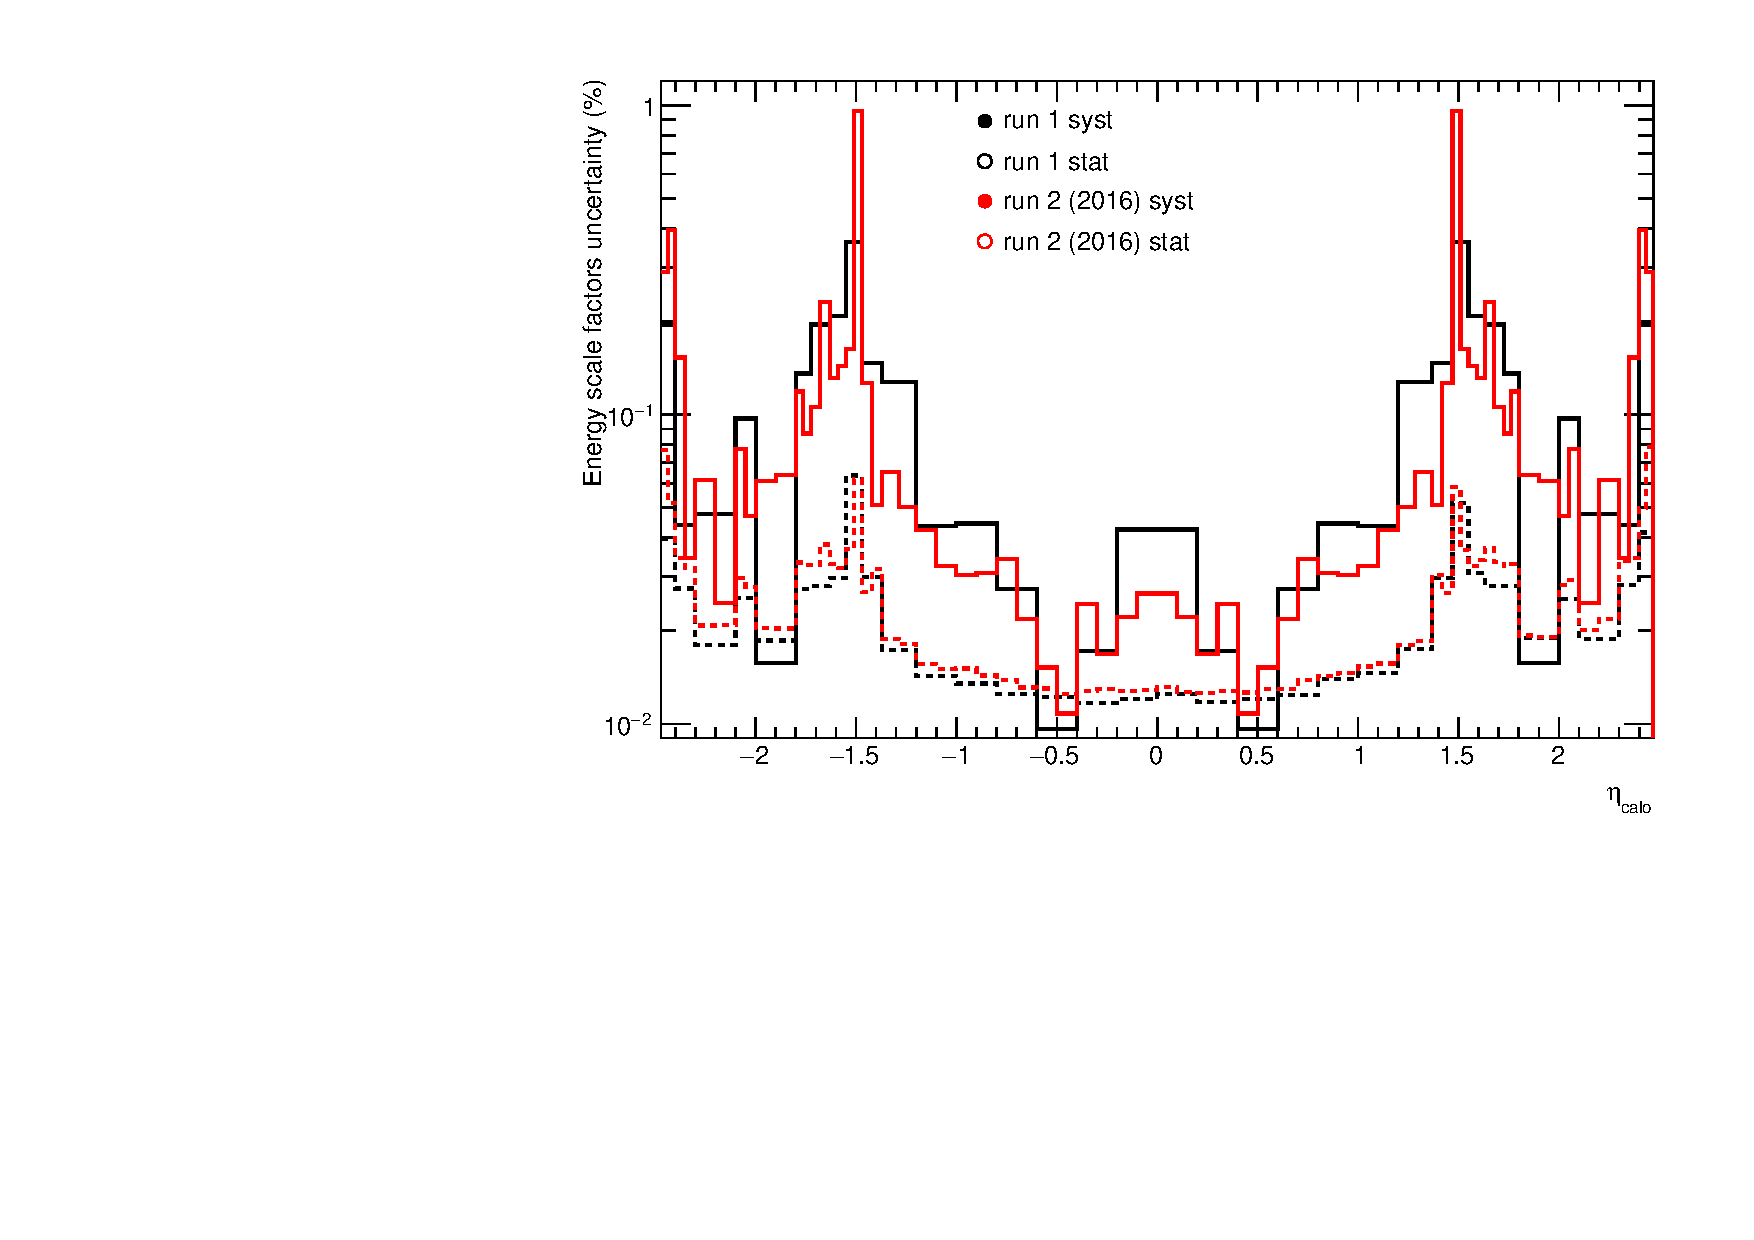
\includegraphics[width=0.9\linewidth]{Figures/CompareSystRun_alpha.pdf}\\
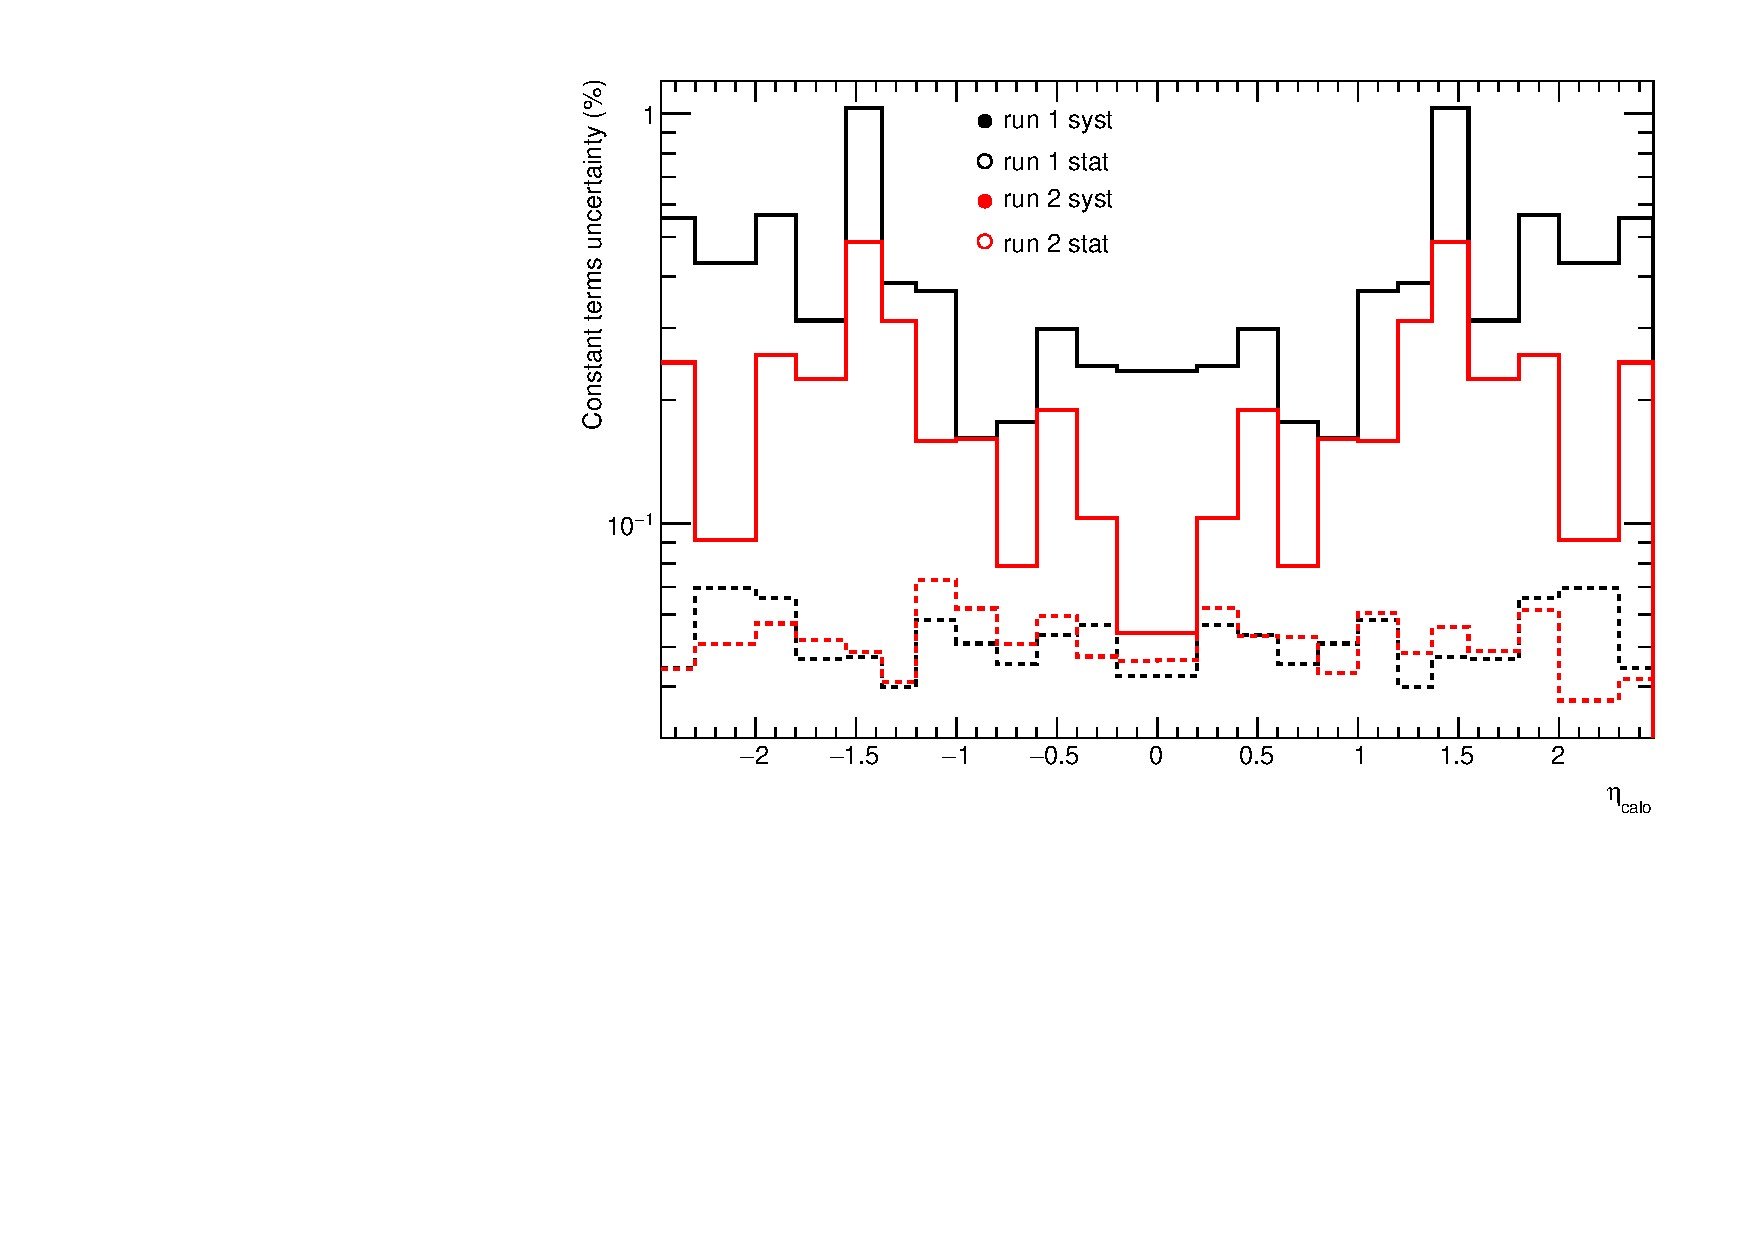
\includegraphics[width=0.9\linewidth]{Figures/CompareSystRun_c.pdf}
\caption{\label{fig:Calibration_CompareScaleRuns}
  Comparison of run 1 and run 2 systematic and statistic uncertainties for the energy scale factors (top) and the resolution constant terms (bottom).
  The statistical uncertainties for the energy scale factors corresponds to the 2016 data while for the constant term the full (2015+2016) run 2 data are used.
}
\end{figure}


\section{Extrapolations}

\subsection{Energy extrapolation}
The in-situ correction assumes that the correction factors only depend on the $\eta$ of the electrons but not on its energy.
Several cross-checks are performed in order to evaluate the residual energy dependence of the scales.

The first test consisted in repeating the same analysis with J/$\Psi$ events decaying into a pair of electrons.
While the $Z$ probes electrons with an average energy of $45$~GeV, the J/$\Psi$ probes much lower energies : around $10$~GeV.
The run 1 study consisted in measuring the residual energy scale factors (as a function of $\eta$) after applying $Z\rightarrow ee$ corrections.
The results, presented in fig. \ref{fig:Calibration_JPsiCheck}, show a bias of the residual scales at low energy at the level of the calibration uncertainties.

\begin{figure}[htbp]
\centering
\includegraphics[width=0.9\linewidth]{CERN-PH-EP-2014-153_30f.pdf}
\caption{\label{fig:Calibration_JPsiCheck}
  Run 1 energy scale factors $\Delta\alpha$ obtained after $Z$- based
  calibration from the $J/\Psi$ sample, as a function of the electron
  pseudorapidity. The band represents the calibration systematic uncertainty. The error bars on the data points represent
  the total uncertainty specific to the $J/\Psi\rightarrow ee$ analysis.
  \cite{CERN-PH-EP-2014-153}}
\end{figure}

A second study has been performed from $Z\rightarrow ee$ events.
It relies on attempting to measure simultaneously the residual energy scale factors as a function of $\eta$ en $E_T$.
$Z$ events must then be further categorised as a function of their electrons $E_T$.
Two possibilities have been implemented and compared :
\begin{enumerate}
\item The matrix method consists in categorising the $Z$ events into a four dimensional matrix indexed by $(\eta_1, \eta_2, E_{T,1}, E_{T,2})$.
  While being the most natural, this method has the drawback of having numerous configurations corresponding to unphysical kinematics.
  Furthermore, the combination of the configurations, which involved a matrix inversion is much more difficult.

\item The summing method consists in labelling the $Z$ as a function of $\eta$ and $E_T$ of a single of its electrons and averaging on the second.
  The event must is then used in two configurations (one per electron) and must be given a weight $1/2$ in order to keep the statistic coherent.
\end{enumerate}
Both method showed similar performances on the MC and were applied to the data.
The difference on the data were slightly larger so the average of both methods have been used as an estimator.
The results are shown in fig. \ref{fig:Calibration_ETDepZ}.
The variations have been considered small and were not corrected.
No similar studies have been performed so far at run 2.
However, a small cross-check of gain (and energy) dependence of the scale have been performed in the context of 2016 diphoton excess (see sec. \ref{sec:calibration_scaleForExcess}) and no significant deviation have been observed.

\begin{figure}[htbp]
\centering
\includegraphics[width=0.7\linewidth]{ATL-COM-PHYS-2013-1653_21fb.pdf}
\caption{\label{fig:Calibration_ETDepZ}
  Run 1 variations of the energy scale as a function of $E_T$ for several $\eta$ bins using $Z\rightarrow ee$ events.
  The central values are the average of two methods using different categorisation (summing or matrix).
\cite{ATL-COM-PHYS-2013-1653}}
\end{figure}


\subsection{Photons extrapolation}

The energy scale factors computed with $Z\rightarrow ee$ events are assumed to be valid also for photons.
Cross-checks have been perform to ensure the validity of the scales for both unconverted and converted photons.
The analysis uses a sample of $Z\rightarrow ll\gamma$ both in the electron and the muonic channels.
The three body invariant mass of the $Z$ is computed in the data by rescaling the photon energy with a test value $\alpha$.
The distribution is then compared to MC and to non-radiative $Z$ mass distribution.
By defining the double ratio
\begin{equation}
  R(\alpha) = \frac{<m(ll\gamma)(\alpha)_\text{data}>/<m(ll)_\text{data}>}{<m(ll\gamma)_\text{MC}>/<m(ll)_\text{MC}>}
\end{equation}
where $<m(ll\gamma)>$ and $<m(ll)>$ are the mean values of the three body and two body invariant masses in the radiative and non-radiative samples, one can determine the most probable value of the parameter $\alpha$ for $R(\hat{\alpha})=1$.
The ratio data/MC allows to remove biases due to the different kinematics in the radiative and non-radiative decays.
The ratio $ll\gamma / ll$ suppresses the leptons energy scale uncertainties.
This measurement have been performed in bins of $\eta$, independently for converted (1 or 2 tracks) and unconverted photons, and is shown (for run 1) in fig. \ref{fig:Calibration_photonScale}.
The observed discrepancies are within the total calibration uncertainties so no additional correction  is performed on the photons.

\begin{figure}[htbp]
\centering
\includegraphics[width=\linewidth]{CERN-PH-EP-2014-153_34f.pdf}
\caption{\label{fig:Calibration_ETDepZ}
  Combined run 1 photon energy scale factors $\Delta\alpha$ obtained after Z -based calibration as a function of $|\eta|$  (left) and $E_T$ (right), for unconverted, one-track converted and two-track converted photons.
  The band represents the calibration systematic   uncertainty.
  The error bars on the data points represent the total uncertainty specific to the $Z\rightarrow ll\gamma$ analyses.
\cite{CERN-PH-EP-2014-153}}
\end{figure}


\section{Material measurement}
\label{sec:orgf6d3909}
The MVA calibration is strongly dependent of the material budget into the detector geometry so a passive material measurement is necessary in order to improve the geometry description and energy resolution.
It relies on the principle of simulating the response of the detector for different geometries \cite{ATL-COM-PHYS-2013-1644} with additional material and compare it to the data.
This additional material has often a constant thickness as a function of z so an incoming electron would cross an increasing amount of matter with increasing $\eta$.
The additional material crossed by a particle, normalised to $X_0$, is then normalised by the shift in E\(_{\text{1/2}}\) it induces in each $\eta$ bin to define a sensitivity factor.
This sensitivity factor ( \(\frac{\partial X/X_0}{\partial E_{1/2}}\) ) is observed to be compatible between all material variations so a common parametrization as a function of $\eta$ is performed, which is presented for electrons and unconverted photons in fig. \ref{fig:orga1f93e3}.
The relative material difference in the data is then computed by multiplying the sensitivity factor with the observed difference of E\(_{\text{1/2}}\) between data and simulation after inter-layer calibration.

This procedure allows to measure the integrated material excess to which a particle is sensitive.
For electrons from Z decay, the material between the interaction point and the L1 is probed.
Using the information from unconverted photons, with a veto on PS activity, the material upstream of the PS can be measured and the difference with the electron results allow to extract the material variation downstream of the PS.
The results of the different cases are presented in fig. \ref{org696c32f}.
The unconverted photons result shows an agreement between the material description in the simulation and the data.
A maximum 5\% discrepancy is observed but covered by the statistical uncertainty on the ID material.
The electrons results display the integrated relative material up to the PS and L1.
Both curves agree in the barrel except for small deviations at $|\eta|<0.9$ and around $|\eta|=0.9$.
Larger discrepancies in the end-cap are observed due to the incomplete SCT heater description.
The agreement of unconverted photons result favours an increase of material in front of the PS.
Material studies on the ID during its construction \cite{ATLASExperiment} show a small $5 \%$ uncertainty, so the material excess is deduced to be a mismodelization of the dead material between the ID and the cryostat.
An improved final run 1 geometry has been defined, correcting for the small discrepancies in the barrel.
Studies are ongoing \cite{ATL-COM-PHYS-2017-759} with run 2 data, on a run 2 geometry that has been slightly improved with respect to the run 1 geometry \cite{141022_Unal}.

\begin{figure}[htbp]
\centering
\includegraphics[width=0.9\linewidth]{CERN-PH-EP-2014-153_19f.pdf}
\caption{\label{fig:orga1f93e3}
Sensitivity factor as a function of $\eta$ for run 1. Only material effect upstream of the PS have been considered for electrons and only after the PS for unconverted photons. Shaded area represent the systematic uncertainty due to the position of the additional material. \cite{CERN-PH-EP-2014-153}}
\end{figure}


\begin{figure}
\begin{subfigure}[t]{.49\linewidth}
\begin{center}
\includegraphics[width=\linewidth]{CERN-PH-EP-2014-153_20fa.pdf}
\end{center}
\end{subfigure}
\begin{subfigure}[t]{.49\linewidth}
\begin{center}
\includegraphics[width=\linewidth]{CERN-PH-EP-2014-153_20fb.pdf}
\end{center}
\end{subfigure}
\caption{\label{org696c32f}
Material difference with respect to the previous geometry as a function of $\eta$ for run 1. Material between PS and L1 is measured using photons with a presampler activity veto. Material integral up to the L1 is measured using electrons. Material integral up to the PS is obtained comparing the two previous results. Error bars include systematic and statistical uncertainties.\cite{CERN-PH-EP-2014-153}}
\end{figure}


\section{Calibration uncertainties}
\label{sec:org76028eb}
The calibration procedure detailed is applied in all analyses on all EM particles.
The impact of calibration on parameters of interest of the various analyses must be evaluated.
In the case of the H\(\rightarrow \gamma \gamma\) coupling analysis, the propagation of the calibration uncertainties is detailed in section \ref{sec:HGam_shapeUncertainties}.
For each calibration step, a number of independent systematic uncertainties are provided as a function of $\eta$ and $p_T$.
In the case of the in-situ correction, one nuisance parameter is defined by the total uncertainty on the constant term and two for the energy scale factors : systematic and statistic.
A set of 80 common nuisance parameters for electrons and photons are defined and five additional related to the conversion status of photons.
Some of the nuisance parameters are related to the same calibration study but are applied in orthogonal $\eta$ bins to decorrelate the effects.

A summary on the contribution of each calibration step in the total scale uncertainty (in relative energy) is presented in fig. \ref{org2897df4} as a function of $\eta$ and $p_T$ for run 1.
One can observe that different systematics are depending on the particle energy, so different analyses will be limited by different effects.
It is important to notice that all scale uncertainty at the exception of the in-situ calibration cancels at $E_T=45$~GeV.
Due to its empirical nature, the in situ calibration absorbs all true systematics effects of the previous calibration steps, hence cancels their uncertainties.

\begin{figure}
  \centering
\begin{subfigure}[t]{0.49\linewidth}
  \includegraphics[width=\linewidth]{CERN-PH-EP-2014-153_29fa.pdf}
  \includegraphics[width=\linewidth]{CERN-PH-EP-2014-153_29fc.pdf}
\end{subfigure}
\begin{subfigure}[t]{0.49\linewidth}
    \includegraphics[width=\linewidth]{CERN-PH-EP-2014-153_29fb.pdf}
    \includegraphics[width=\linewidth]{CERN-PH-EP-2014-153_29fd.pdf}
\end{subfigure}
\caption{\label{org2897df4}
  Breakdown of run 1 calibration uncertainties as a function of $E_T$ for electrons (top) and unconverted photons (bottom). \cite{CERN-PH-EP-2014-153}}
\end{figure}

The contribution of various sources of uncertainty to the relative total uncertainty on the resolution is given in fig. \ref{fig:Calibration_totResUnc} for electrons and unconverted photons.

\begin{figure}[htbp]
\centering
\includegraphics[width=\linewidth]{CERN-PH-EP-2014-153_36f.pdf}
\caption{\label{fig:Calibration_totResUnc}
  Contributions of the different uncertainties to the relative resolution uncertainty as a function of $E_T$ for electrons (left) and unconverted photons (right) with $|\eta|=0.2$.
  \cite{CERN-PH-EP-2014-153}}
\end{figure}
